\section{Attēlu raksturpunkti} \label{sec:algo}
Attēla \newTerm{raksturpunkti} (\termEn{features}) ir attēla punktu (pikseļu)
apakškopa kuri paši, vai biežāk to apkārtne attēlā 
satur (vai potenciāli satur) noderīgu informāciju mašīnredzes algoritmiem.
Raksturpunktus ļoti bieži atlasa ar ,,stūru meklēšanas'' algoritmu,
tāpēc literatūrā vārdi ,,raksturpunkts'' (\termEn{feature point}) un ,,stūris''
(\termEn{corner}) bieži tiek izmantoti kā sinonīmi. Piemēram, dažādu attēlu
raksturpunktu salāgošanas algoritmam --- kāds ir apskatīts šajā darbā ---
ir nozīmīga raksturpunktu apkārtnes unikalitāte,
lai raksturpunktus būtu iespējams salāgot ar pēc iespējas mazāk kļūdām,
nevis to strikta atbilstība attēla objekta stūrim.

Galvenais pamatojums attēlu raksturpunktu atlasei, ir nepieciešamās
skaitļošanas apjoma samazināšanai atmetot (potenciāli) nelietderīgo
skaitļošanu. Sevišķi svarīgi tas ir augstas kompleksitātes algoritmiem,
kuriem nepieciešamā skaitļošanas jauda krasi pieaug palielinoties
elementu skaitam. Otrs apsvērums, ir ka algoritmi kas izstrādāti balstoties
uz raksturpunktiem var dot neadekvātus rezultātus ja tiek apskatīti visi
attēla punkti.

\subsection{Attēlu raksturpunktu pāru atrašanas algoritmi} \label{sec:matching}
\begin{figure}[tbh]
	\centering
	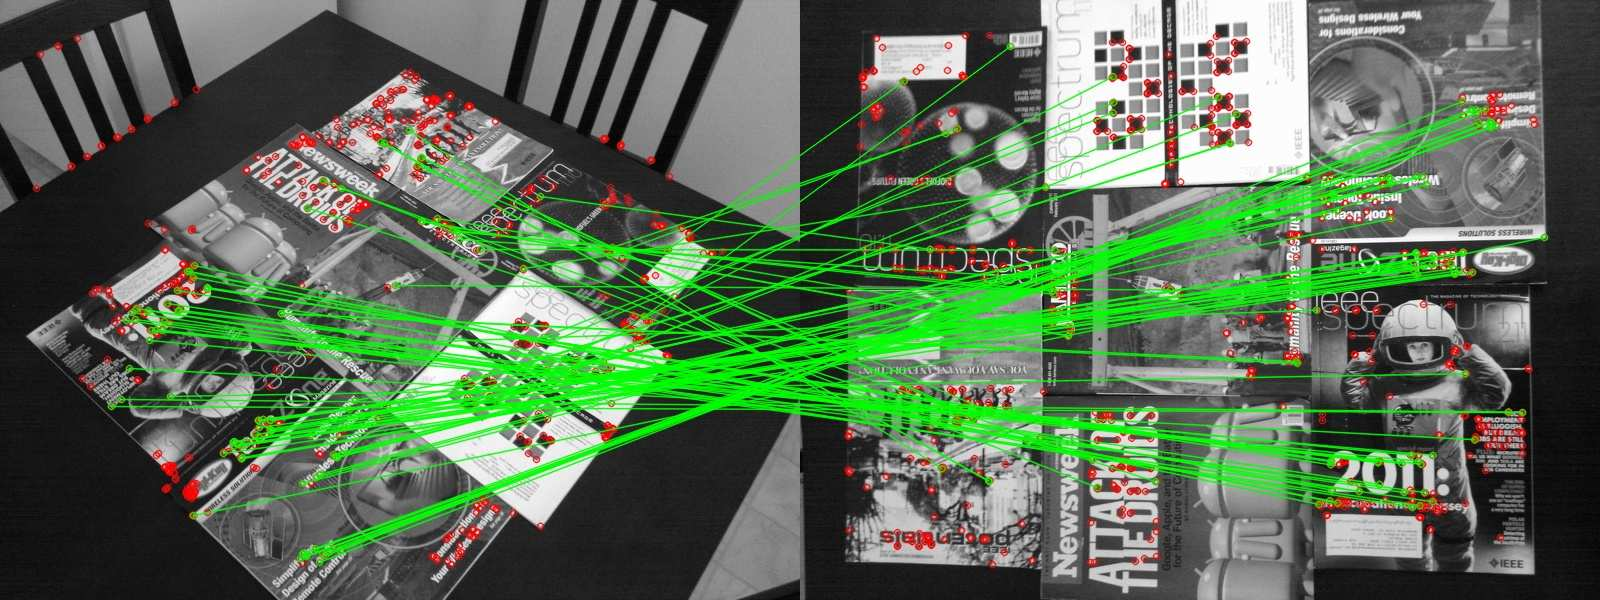
\includegraphics[width=0.8\textwidth]{orb-match}
	\caption{Divu attēlu atbilstošo raksturpunktu pāru noteikšana ar ORB~\cite{ORB}.}
	\label{fig:orb}
\end{figure}

Raksturpunktu pāru atrašanas ir atbilstošo punktu atrašana divos
(vai vairākos) attēlos, kuri atbilst vienam un tam pašam attēlā redzamam
objektam. Piemērs redzams \ref{fig:orb}~attēlā, kur ar zaļām līnijām
savienoti atrastie raksturpunktu pāri un ar sarkanu apzīmēti raksturpunkti,
kuriem pāris nav atrasts.

Raksturpunktu pāru noteikšana tiek izmantota tādos mašīnredzes pielietojumos, kā
% TODO: citēt pielietojumus
objektu atpazīšanā un sekošanā, attēlu ,,sašūšanā'', 
telpiskās informācijas rekonstrukcijā (kartēšanā) no attēliem,
vienlaicīgā pašlokalizācijā un kartēšanā (SLAM), u.c..

Raksturpunktu pāru noteikšanas pamatā ir šo punktu ,,aprakstīšana'' izveidojot
raksturpunkta \newTerm{deskriptoru}, kas satur informāciju,
kas ir pietiekami unikāla, lai nesakristu ar citiem raksturpunktiem attēlā
un ir noturīga pret sagaidāmām attēla īpašību izmaiņām, un to salāgošana
atrodot līdzīgos deskriptoru pārus.
Deskriptoram tātad nepieciešamas vai vēlamas šādas īpašības:
\begin{itemize}
	\item \newTerm{\emph{diskriminitāte}} --- spēja izšķirt raksturpunktus
		pēc to deskriptoriem;
	\item \emph{pozīcijas invariance} --- spēja salāgot raksturpunktus
		neatkarīgi no tā koordinātēm attēlā;
	\item \emph{rotācijas invariance} --- spēja salāgot raksturpunktus
		neatkarīgi no attēla rotācijas leņķa;
	\item \emph{intensitātes nobīdes invariance} --- spēja salāgot raksturpunktus
		neatkarīgi no globālas intensitātes izmaiņas;
	\item \emph{mēroga invariance} --- spēja salāgot raksturpunktus
		neatkarīgi no mēroga (attēla izmēru un/vai raksturpunkta objekta attāluma izmaiņa);
	\item \emph{perspektīvas invariance} --- spēja salāgot raksturpunktus
		neatkarīgi no perspektīvas (attēla uzņemšanas pozīcijas izmaiņa);
	\item \emph{trokšņu noturība} --- spēja salāgot raksturpunktus
		attēlā (iespējami) neatkarīgi no ,,trokšņa'' līmeņa attēlā;
\end{itemize}
Ir norādītas vairākas attēla izmaiņu invariances īpašības,
kas nozīmē, ka šī informācija nav izmantojama,
lai aprakstītu raksturpunktu.
Variance ir nepieciešama, lai nodrošinātu diskriminitāti un, praktiski visos
algoritmos, tiek izmantota lokālas intensitātes izmaiņas attēlā 
rakturpunkta tuvējā apkārtnē.

Eksistē vairāki algoritmi deskriptoru izgūšanai un
salīdzināšanai, t.sk.,~%
SIFT, % FIXME: Vai SIFT arī apzīmē deskriptoru?
SURF, BRIEF un tā varianti, ORB, u.c..
Algoritmus var izvērtēt pēc jau uzdotajām īpašībām, 
bet jāņem vērā arī to veiktspējas īpašības:
\begin{itemize}
	\item \emph{skaitļošanas kompleksitāte}, kas tieši ietekmē algoritma
		ātrdarbību;
	\item \emph{informācijas blīvums}, kas atspoguļo cik liela ir katra
		informācijas bita variance, kas ļauj sasniegt lielāku diskriminitāti
		pie mazāka bitu skaita.
\end{itemize}
% TODO?: Izvērst dažādo algoritmu teorētisko aprakstu?

Netiešs, bet būtisks, pāru noteikšanas ietekmējošais faktors ir 
labu raksturpunktu
atlase no attēla, jo salāgošana tiek veikta tikai starp atlasītajiem
punktiem. Raksturpunktu (un to detektēšanas algoritmu) galvenās īpašības
ir to variance, kas nosaka cik aprakstoši ir šie punkti,
un \newTerm{atkārtojamība}, kas izsaka atbilstošo punktu pāru piederību
raksturpunktu kopai dažādos attēlos pret kopējo raksturpunktu skaitu~%
\cite{FAST}\cite{SIFT-FPGA}.
Raksturpunktu atlases algoritmi un to īpašības plašāk apskatītas
\ref{sec:corners}~apakšnodaļā.

Šajā darbā, turpmākai algoritma implementāciju veiktspējas izvērtēšanai
un salīdzināšanai izvēlēts, ORB algoritms, vai konkrētāk tā salāgošanas
komponente --- rBRIEF.
% TODO: Forward ref
Šāda izvēle pamatota ar to, ka rBRIEF raksturpunktu salāgošanas
spēja ir līdzīga vai labāka nekā SIFT, bet ir par divām kārtām ātrāks nekā
SIFT un par kārtu ātrāks nekā SURF \cite{ORB}.
rBRIEF deskriptors ir arī noturīgāks pret troksni nekā
SIFT un tā rotācijas invariance līdzvērtīga SIFT \cite{ORB}.



